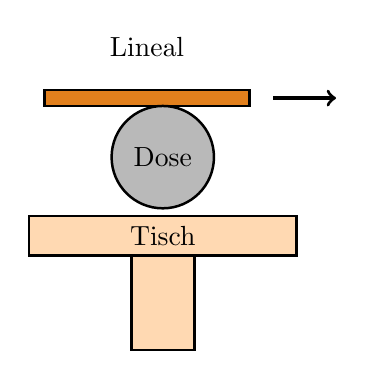
\begin{tikzpicture}[line width=0.9pt]
  % ruler "Lineal"
  \node[above] at (-0.7,2.0) {Lineal};
  \draw[fill=orange!55!brown, draw=black] (-2.0,1.5) rectangle (0.6,1.7);
  % arrow indicating ruler motion
  \draw[->, line width=1.2pt] (0.9,1.6) -- (1.7,1.6);
  % disc "Dose"
  \draw[fill=gray!55, draw=black] (-0.5,0.85) circle (0.65);
  \node at (-0.5,0.85) {Dose};
  % table "Tisch" (T-shape)
  \draw[fill=orange!30, draw=black] (-2.2,-0.4) rectangle (1.2,0.1);
  \draw[fill=orange!30, draw=black] (-0.9,-1.6) rectangle (-0.1,-0.4);
  \node at (-0.5,-0.15) {Tisch};
\end{tikzpicture}
